\documentclass[tikz,border=14pt]{standalone}
\usepackage[T1]{fontenc}
\usepackage{tgheros}
\usepackage{sfmath}
\usepackage{amsmath}
% % \usepackage{fontawesome5} (Removed for publication-grade academic typography) (Removed for publication-grade academic typography)
\usepackage{tikz}
\usetikzlibrary{arrows.meta,positioning,shapes.geometric,fit,backgrounds,calc}
\usepackage{xcolor}

\renewcommand{\familydefault}{\sfdefault}

% Academic Semantic Palette
\definecolor{harvardcrimson}{HTML}{A51C30}
\definecolor{ethdarkblue}{HTML}{1F407A}
\definecolor{ethblue}{HTML}{215CAF}
\definecolor{ethpetrol}{HTML}{007A87}
\definecolor{ethbronze}{HTML}{B87333}
\definecolor{ethslate}{HTML}{475569}
\definecolor{cardbg}{HTML}{F8FAFC}
\definecolor{cardborder}{HTML}{CBD5E1}
\definecolor{safeTeal}{HTML}{10B981}
\definecolor{warnAmber}{HTML}{D97706}
\definecolor{coralRed}{HTML}{DC2626}

\begin{document}
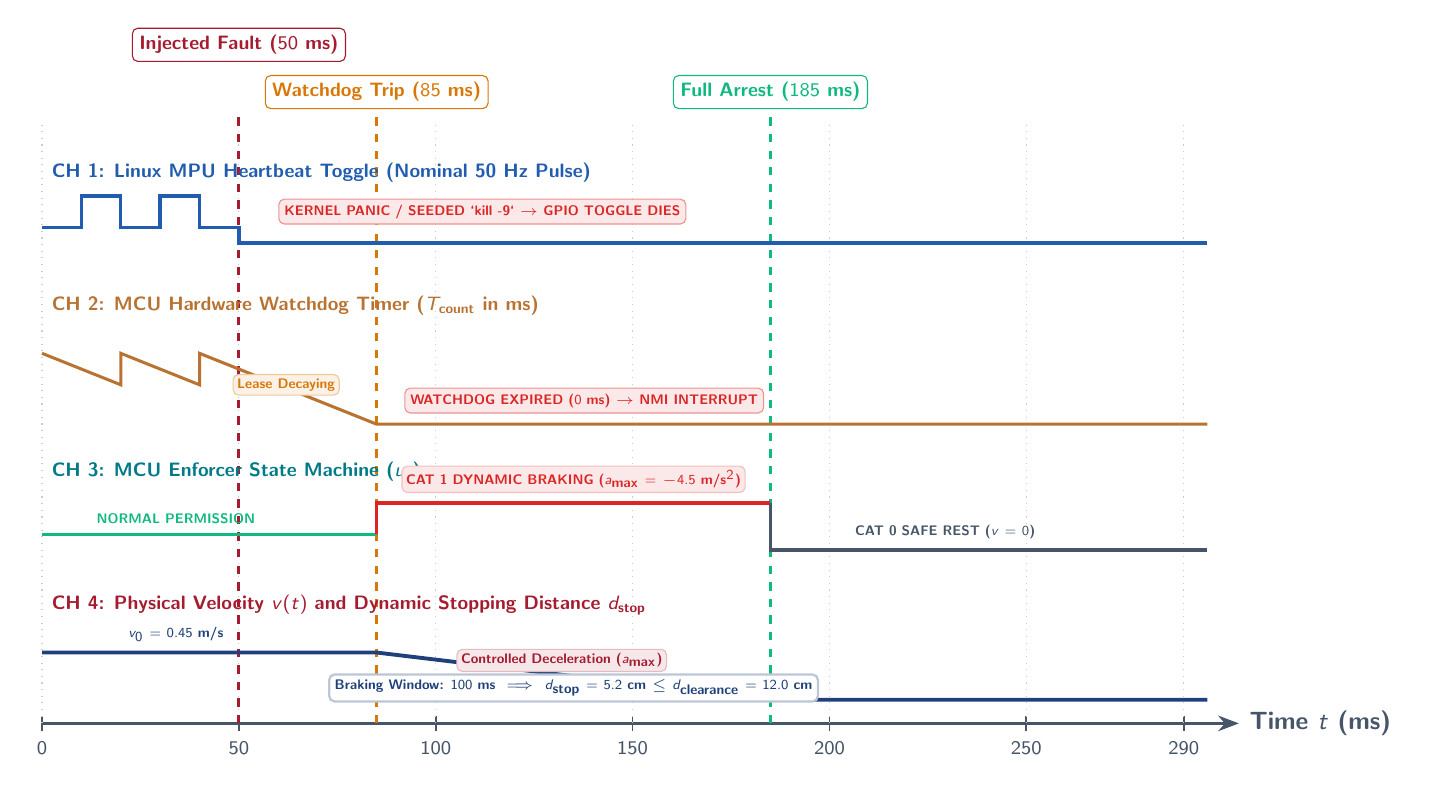
\begin{tikzpicture}[
  font=\sffamily,
  >=Stealth
]



  % Time Axis (Bottom)
  \draw[->, line width=1.0pt, ethslate] (0, 0) -- (15.2, 0) node[right, font=\sffamily\small\bfseries] {Time $t$ (ms)};
  
  \foreach \x/\label in {0/0, 2.5/50, 5.0/100, 7.5/150, 10.0/200, 12.5/250, 14.5/290} {
    \draw[line width=0.6pt, ethslate] (\x, 0.1) -- (\x, -0.1) node[below, font=\sffamily\scriptsize] {\label};
    \draw[dotted, line width=0.4pt, ethslate!30] (\x, 0) -- (\x, 7.6);
  }

  % Critical Vertical Markers (Clean non-overlapping headers)
  % 1. Fault Injection: t = 50 ms (x = 2.5)
  \draw[line width=1.1pt, harvardcrimson, dashed] (2.5, 0) -- (2.5, 7.8);
  \node[font=\sffamily\scriptsize\bfseries, fill=white, draw=harvardcrimson, rounded corners=2pt, inner sep=2.5pt, text=harvardcrimson, anchor=south] at (2.5, 8.4) {
     Injected Fault ($50\text{ ms}$)
  };

  % 2. Watchdog Expiry: t = 85 ms (x = 4.25)
  \draw[line width=1.1pt, warnAmber, dashed] (4.25, 0) -- (4.25, 7.8);
  \node[font=\sffamily\scriptsize\bfseries, fill=white, draw=warnAmber, rounded corners=2pt, inner sep=2.5pt, text=warnAmber, anchor=south] at (4.25, 7.8) {
     Watchdog Trip ($85\text{ ms}$)
  };

  % 3. Full Arrest: t = 185 ms (x = 9.25)
  \draw[line width=1.1pt, safeTeal, dashed] (9.25, 0) -- (9.25, 7.8);
  \node[font=\sffamily\scriptsize\bfseries, fill=white, draw=safeTeal, rounded corners=2pt, inner sep=2.5pt, text=safeTeal, anchor=south] at (9.25, 7.8) {
     Full Arrest ($185\text{ ms}$)
  };

  % ----------------------------------------------------
  % TRACE 1: Linux MPU Heartbeat (GPIO Toggle)
  % ----------------------------------------------------
  \node[anchor=west, font=\sffamily\scriptsize\bfseries, text=ethblue] at (0, 7.0) {
     CH 1: Linux MPU Heartbeat Toggle (Nominal 50 Hz Pulse)
  };
  \draw[line width=1.2pt, ethblue] 
    (0, 6.3) -- (0.5, 6.3) -- (0.5, 6.7) -- (1.0, 6.7) -- (1.0, 6.3) -- (1.5, 6.3) -- (1.5, 6.7) -- (2.0, 6.7) -- (2.0, 6.3) -- (2.5, 6.3)
    -- (2.5, 6.1) -- (14.8, 6.1);
  \node[font=\sffamily\tiny\bfseries, fill=coralRed!10, text=coralRed, draw=coralRed!50, rounded corners=2pt, inner sep=2pt, anchor=west] at (3.0, 6.5) {
    KERNEL PANIC / SEEDED `kill -9` $\to$ GPIO TOGGLE DIES
  };

  % ----------------------------------------------------
  % TRACE 2: Hardware Watchdog Countdown Value
  % ----------------------------------------------------
  \node[anchor=west, font=\sffamily\scriptsize\bfseries, text=ethbronze] at (0, 5.3) {
     CH 2: MCU Hardware Watchdog Timer ($T_{\text{count}}$ in ms)
  };
  \draw[line width=1.1pt, ethbronze]
    (0, 4.7) -- (1.0, 4.3) -- (1.0, 4.7) -- (2.0, 4.3) -- (2.0, 4.7) -- (2.5, 4.5)
    -- (4.25, 3.8)
    -- (14.8, 3.8);
  \node[font=\sffamily\tiny\bfseries, fill=warnAmber!10, text=warnAmber, draw=warnAmber!40, rounded corners=2pt, inner sep=1.5pt] at (3.1, 4.3) {Lease Decaying};
  \node[font=\sffamily\tiny\bfseries, fill=coralRed!10, text=coralRed, draw=coralRed!50, rounded corners=2pt, inner sep=2pt, anchor=west] at (4.6, 4.1) {
    WATCHDOG EXPIRED ($0\text{ ms}$) $\to$ NMI INTERRUPT
  };

  % ----------------------------------------------------
  % TRACE 3: MCU Enforcer Authority State Machine
  % ----------------------------------------------------
  \node[anchor=west, font=\sffamily\scriptsize\bfseries, text=ethpetrol] at (0, 3.2) {
     CH 3: MCU Enforcer State Machine ($u_t$)
  };
  \draw[line width=1.3pt, safeTeal] (0, 2.4) -- (4.25, 2.4) 
    node[pos=0.4, above, font=\sffamily\tiny\bfseries, text=safeTeal] {NORMAL PERMISSION};
  \draw[line width=1.3pt, coralRed] (4.25, 2.4) -- (4.25, 2.8) -- (9.25, 2.8);
  \node[font=\sffamily\tiny\bfseries, fill=coralRed!10, text=coralRed, draw=coralRed!30, rounded corners=2pt, inner sep=1.5pt] at (6.75, 3.1) {
    CAT 1 DYNAMIC BRAKING ($a_{\text{max}}=-4.5\text{ m/s}^2$)
  };
  \draw[line width=1.3pt, ethslate] (9.25, 2.8) -- (9.25, 2.2) -- (14.8, 2.2) 
    node[pos=0.4, above, font=\sffamily\tiny\bfseries, text=ethslate] {CAT 0 SAFE REST ($v=0$)};

  % ----------------------------------------------------
  % TRACE 4: End-Effector Physical Velocity & Stopping Margin
  % ----------------------------------------------------
  \node[anchor=west, font=\sffamily\scriptsize\bfseries, text=harvardcrimson] at (0, 1.5) {
     CH 4: Physical Velocity $v(t)$ and Dynamic Stopping Distance $d_{\text{stop}}$
  };
  \draw[line width=1.4pt, ethdarkblue] 
    (0, 0.9) -- (4.25, 0.9) node[pos=0.4, above, font=\sffamily\tiny\bfseries] {$v_0 = 0.45\text{ m/s}$}
    -- (9.25, 0.3)
    -- (14.8, 0.3);

  \node[font=\sffamily\tiny\bfseries, fill=harvardcrimson!10, text=harvardcrimson, draw=harvardcrimson!30, rounded corners=2pt, inner sep=1.5pt] at (6.6, 0.8) {
    Controlled Deceleration ($a_{\text{max}}$)
  };

  % Stopping Distance Margin Bracket
  \draw[<->, line width=0.8pt, ethdarkblue] (4.25, 0.45) -- (9.25, 0.45)
    node[midway, fill=white, draw=ethdarkblue!30, rounded corners=2pt, inner sep=2pt, font=\sffamily\tiny\bfseries, text=ethdarkblue] {
      Braking Window: $100\text{ ms} \implies d_{\text{stop}} = 5.2\text{ cm} \le d_{\text{clearance}} = 12.0\text{ cm}$
    };

\end{tikzpicture}
\end{document}
